\documentclass[a4paper, 11pt]{article}
 
\usepackage[utf8]{inputenc}
\usepackage{graphicx}
\usepackage[frenchb]{babel}
\usepackage{makecell}
\usepackage{listings}
\usepackage[dvipsnames]{xcolor}

\lstset{language=C,
	 	basicstyle=\ttfamily,
		keywordstyle=\ttfamily\textcolor{RubineRed},
		identifierstyle=,columns=fullflexible,
		commentstyle=\textcolor{OliveGreen},
		showstringspaces=false, breaklines=true,tabsize=4}

\begin{document}
 
\title{Compilation Avanc\'ee\\Devoir de programmation - ML2C}
\author{Ilyas Toumlilt}
\date{12/03/2015}
 
\maketitle
 
\paragraph{Introduction :} Compilation d'un langage fonctionnel - Bibliothèque d'éxecution.\\
\textit{``La principale difficult\'e de la mise en oeuvre d'un langage fonctionnel vient de la traduction du contr\^ole implicite de l'\'execution dans un mod\`ele de calcul o\`u il devient explicite.''}\\
L'objectif de ce projet est la traduction d'un langage fonctionnel ( OCaml ) en langage impératif, le choix du langage cible s'est fait au ``top of mind'', le langage C.\\
La réalisation du projet s'inspire de celle vue en TD et fournie avec ce projet, ML2Java.

\paragraph{Fichiers inclus} :\\
\textbf{/} : est la racine du projet.\\
\textbf{/fournis} : contient les fichiers fournis pour le projet, en l'occurrence ML2Java.\\
\textbf{/src} : contient les sources du projet ML2C, dont particulièrement :\\
\textbf{/src/runtime.h} : la bibliothèque d'éxecution C. ( définition )\\
\textbf{/src/runtime.c} : la bibliothèque d'éxecution C. ( implémentation )\\
\textbf{/src/Makefile} : make des commandes de compilation et génération du compilateur ml2c.\\
\textbf{/src/prod.ml} : le traducteur LI vers C.\\
\textbf{/src/trans.ml} : le traducteur vers LI.\\
\textbf{/src/eval.ml} : évaluateur.\\
\textbf{/src/ftest.ml} : fichier de test fournis.\\
\textbf{/src/*} : le reste des fichiers ne changent pas de ceux de la réalisation ML2Java.\\
Le C ( tout comme le Java ), nous permettera d'avoir une bibliothèque d'éxecution très réduite.

\paragraph{Organisation de ML2C} :\\
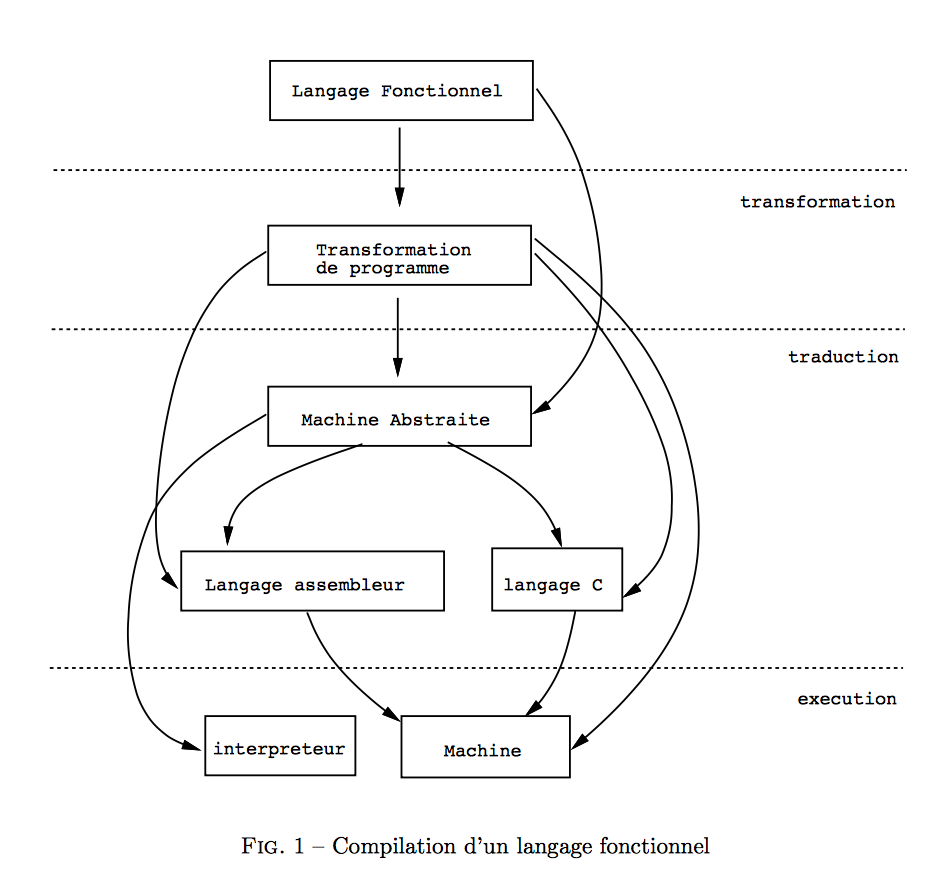
\includegraphics[scale=0.7]{organisation.png}

\paragraph{Biblioth\`eque d'\'execution } :\\
Cette bibliothèque représente les types ML comme instances de la structure MLvalue, cette structure contient deux champs, le type un entier identifiant de manière unique chaque type ML ( voir defines runtime.h ), et le contenu qui est représenté comme une union traduisant les différents tyes représentés.
\begin{lstlisting}
struct _MLvalue {
  int type; /* takes a value from defines above */
  union {   /* value's content */
    int MLunit;
    int MLint;
    int MLbool;
    double MLdouble;
    char* MLstring;
    struct _MLpair {
      MLvalue *MLfst, *MLsnd;
    } MLpair;
    struct _MLlist {
      MLvalue *MLcar;
      MLvalue *MLcdr;
    } *MLlist;
    struct _MLfun {
      int counter;
      int nbparams;
      MLvalue** env;
      MLvalue* (*invoke)(MLvalue*, MLvalue*);
    } MLfun;
  };
};
\end{lstlisting}

Chaque type ML est construit grace à une fonction ``d'instanciation'' ( nommées makeML<type> ), par exemple un entier et construit comme ceci :
\begin{lstlisting}
  MLvalue* newMLint(int v)
  {
    MLvalue* r = (MLvalue*)malloc(sizeof(MLvalue));
    r->type    = MLINT;
    r->MLint   = v;
    return r;
  }
\end{lstlisting}

Tous les autres types de bases sont construits de la sorte, à l'exception des types fonctionnels. Les valeurs des types fonctionnels correspondent aux fermetures de ML, le type MLfun se construit ainsi :
\begin{lstlisting}
  MLvalue* newMLfun(MLvalue *f, int c, MLvalue* (*invoke)(MLvalue*, MLvalue*))
  {
    MLvalue* r = (MLvalue*)malloc(sizeof(MLvalue));
    r->type    = MLFUN;
    int i;
    if(f){
      r->MLfun.nbparams = f->MLfun.nbparams;
      r->MLfun.counter  = c;
      r->MLfun.env      = (MLvalue**)malloc(sizeof(MLvalue*));
      for(i=0; i<c; i++)
      r->MLfun.env[i] = NULL;
      if(f->MLfun.env)
      memcpy(r->MLfun.env, f->MLfun.env,
      f->MLfun.counter*(sizeof(MLvalue)));
      r->MLfun.invoke = f->MLfun.invoke;
    } else {
      r->MLfun.nbparams = c;
      r->MLfun.counter  = 0;
      r->MLfun.env      = NULL;
      r->MLfun.invoke   = invoke;
    }
    return r;
  }
\end{lstlisting}

\paragraph{Production du code C} : \\
Un programme ML est traduit à la phase précédente par une liste d'instructions du langage intérmédiaire. La production du code C s'effectue en trois passes qui chacune parcourt cette liste. La première récupère toutes les définitions de fonctions et produit les instances de structures C équivalentes. La deuxième effectue les déclarations globales des fonctions, des variables globales non fonctionnelles et des noms associés aux expressions globales. Enfin la troisième passe écrit la fonction main correspondant aux différentes expressions globales rencontrées dans le programme. Ces trois passes se retrouvent dans le fichier prod.ml. On peut aisément imaginer de traduire ce langage intérmédiaire vers un autre langage.

\paragraph{Exemple de compilation} : \\
Le fichier fourni /src/ftest.ml implémente quelques opération ml de base, sa compilation avec ml2c produit /src/ftest.c, un premier reflèxe serait de comparer les sorties des deux compilations ( ml2java vs ml2c ), le résultat est exactement le même.

\end{document}
